\section{流水线与并行处理的基本模型}\label{co-ch6}

\subsection{延迟和完成间隔是两个量}\label{co-06-01}

把一条指令分为 k 段，每段使用自己的部件或使用时段，让多条指令的不同阶段重叠执行，称为指令流水线。流水线没有让同一条指令的先后依赖消失：必须先取得地址，才能读取相应数据。它主要提高连续指令的吞吐率。

理想 k 段流水线，每段耗时一个时钟周期 \(\tau\)，无停顿且一次每周期启动一条指令，完成 n 条指令需

\[
T_{\mathrm{pipe}}=(k+n-1)\tau.
\]

前 k 个周期使第一条指令通过全线，此后每周期再完成一条。不是每条都额外支付一次填充时间。吞吐率为 \(n/T_{\mathrm{pipe}}\)，n足够大时趋近 \(1/\tau\)；单条延迟约为 \(k\tau\)。加入停顿 s 周期后，总时间变为 \((k+n-1+s)\tau\)，前提是按本模型每个停顿周期使最终完成时间增加一周期。

若非流水方案每条确实依次完成这 k 段、每段也用同样的 \(\tau\)，则非流水时间为 \(nk\tau\)，加速比为 \(nk/(k+n-1)\)。若原方案时钟不同、可以不等长执行或另有资源复用，要重新计算基线，不能直接把流水级数当加速比。

\subsubsection{例 6-1　最慢的一段决定时钟下限}\label{co-ex6-1}

\noindent{}【2009】 某计算机的指令流水线由四个功能段组成，指令流经各功能段的时间（忽略各功能段之间的缓存时间）分别为90 ns、80 ns、70 ns和60 ns，则该计算机的 CPU 时钟周期至少是（　）。

A. 90 ns　 B. 80 ns　 C. 70 ns　 D. 60 ns

\Needspace{6\baselineskip}

\textbf{解析。} 相邻阶段寄存器在同一节拍推进，必须留足最慢段90 ns，选 \textbf{A}。若实际阶段寄存器开销为 \(t_r\)，则通常需至少 \(\max_i(t_i)+t_r\)，题目已说忽略这项。

在本题时间下，理想完成10条指令需 \((4+10-1)\times90=1170\) ns。若非流水方案每条直接耗时 \(90+80+70+60=300\) ns，10条为3000 ns，加速比约2.56；若基线规定每段都占90 ns，又得到另一基线时间。比较时必须明确分母采用哪种机器。

\subsection{阶段寄存器保存的不只是一份数据}\label{co-06-02}

五段教学流水线常写为 IF取指、ID译码/寄存器读、EX执行或地址计算、MEM访存、WB写回。算术指令也可能经过MEM这一拍但不访问数据存储器；存储指令通常不在WB写通用寄存器。阶段名描述某种通路设计，不是每条指令都在每段做同一种事。

阶段之间的寄存器保存下一段所需的操作数、立即数、目的寄存器编号、指令地址及控制信息。若只传数据不传目的编号，结果就可能写到错误寄存器；若指令阻塞时仍让其写使能继续流动，也可能重复写入或错误访存。

时钟推进状态，控制信号决定状态写入是否允许及组合部件选择什么功能。阶段寄存器常需写使能、保持和清空控制，因此``控制仅作用于组合部件、时钟仅作用于寄存器''的割裂描述不能当作普遍规则。气泡是在某阶段放入不产生有效状态改变的操作，冻结是让原状态保留，两者效果不同。

\subsection{冒险先按冲突对象分类}\label{co-06-03}

结构冒险来自同拍争用不足的硬件资源。例如取指和数据读取同时需要单端口统一存储器；可通过停顿、增加端口或分离指令与数据存储来处理。寄存器组同拍读写是否冲突，取决于端口数及前后半拍的时序约定。

数据冒险来自指令间数据依赖与执行时序的矛盾。写后读 RAW：后指令读前指令产生的新值；读后写 WAR：后指令过早写破坏前指令尚未读取的旧值；写后写 WAW：两次写的完成顺序颠倒，使最终值错误。在固定五段、顺序发射、ID读寄存器且WB顺序写回的简单流水线中，通常需要处理RAW，而WAR、WAW被既定次序排除。变为乱序执行或不同延迟写回后，这个结论不再普遍成立。

控制冒险来自后继指令地址未确定，常见于条件分支、跳转、异常和中断处理。无条件转移仍需在某个时刻获得目标地址，因而也可能造成前端控制冒险。不能因为``不判断条件''便断言``不会停顿''。

\subsubsection{转发能省去等待写回，但不能送来尚未产生的数据}\label{ux8f6cux53d1ux80fdux7701ux53bbux7b49ux5f85ux5199ux56deux4f46ux4e0dux80fdux9001ux6765ux5c1aux672aux4ea7ux751fux7684ux6570ux636e}

转发把已经形成的结果从阶段寄存器等位置直接送到后续指令使用点，不必等写回寄存器组。例如ALU结果在EX结束时产生，后继指令下一拍进入EX，可以从EX/MEM处取得它。

load的数据通常到MEM结束才产生。紧随其后的指令若下一拍EX就需要该值，即使有转发也来不及，必须插入一个等待周期。转发路径是否通往存储数据端、分支比较端，也要看图，不能看见``支持转发''就推断所有相关都已解决。

\subsubsection{同一组RAW，在不同实现中等到哪一拍}\label{ux540cux4e00ux7ec4rawux5728ux4e0dux540cux5b9eux73b0ux4e2dux7b49ux5230ux54eaux4e00ux62cd}

\begin{longtable}[]{@{}
  >{\raggedright\arraybackslash}p{(\columnwidth - 4\tabcolsep) * \real{0.3056}}
  >{\raggedright\arraybackslash}p{(\columnwidth - 4\tabcolsep) * \real{0.3437}}
  >{\raggedright\arraybackslash}p{(\columnwidth - 4\tabcolsep) * \real{0.3505}}@{}}
\toprule\noalign{}
\begin{minipage}[b]{\linewidth}\raggedright
题设实现
\end{minipage} & \begin{minipage}[b]{\linewidth}\raggedright
消费者取得值的条件
\end{minipage} & \begin{minipage}[b]{\linewidth}\raggedright
排时序时使用的约束
\end{minipage} \\
\midrule\noalign{}
\endhead
\bottomrule\noalign{}
\endlastfoot
无转发，寄存器同拍不能读写 & 必须等生产者WB结束，再在ID读 & 消费者ID至少比生产者WB晚1拍 \\
无转发，寄存器同拍先写后读 & 生产者WB前半拍写，消费者ID后半拍读 & 可以让消费者ID与生产者WB同拍 \\
ALU结果向EX转发 & 生产者EX末已有结果，下一拍送消费者EX & 不必为该值等到寄存器WB \\
load结果向EX转发 & 生产者MEM末才有读出数据 & 消费者EX须在该MEM之后，紧邻load仍可能停1拍 \\
\end{longtable}

``相关''由程序中谁产生、谁使用同一个值决定；``冒险是否导致停顿''还由结果产生点、使用点、转发路径和寄存器时序共同决定。因此，无转发题不能套下面load-use的一拍结论，有转发题也不能机械等到所有源都WB。STORE的数据可能在ID读取、在MEM使用，分支可能在ID或EX比较，须先读具体通路约定。

\subsubsection{例 6-2　装入后立即使用需要一个气泡}\label{co-ex6-2}

\noindent{}〖5.6-013〗 下列指令序列中，指令I1和I3、I2和I3之间发生数据相关。假定采用``取指、译码/取数、执行、访存、写回''五段流水线方式，那么在采用转发技术时，需要在指令I3之前加入（　）条空操作指令才能使这段程序不发生数据冒险。

\par\medskip\noindent
\begin{minipage}{\linewidth}
\begin{verbatim}
I1: add  r1, r0, 1    // R[r1] <- R[r0] + 1
I2: load r3, 12(r2)   // R[r3] <- M[R[r2] + 12]
I3: add  r5, r3, r1   // R[r5] <- R[r3] + R[r1]
\end{verbatim}
\end{minipage}\par\medskip

A. 3　 B. 2　 C. 0　 D. 1

\Needspace{6\baselineskip}

\textbf{解析。} I1在第3拍EX末形成r1结果，到I3需要时已经可用；I2到第5拍MEM末才有r3数据，而无停顿的I3本应在第5拍EX使用它，时间相撞。把I3的EX推迟到第6拍即可，因此选 \textbf{D}。

\begin{figure}
\centering
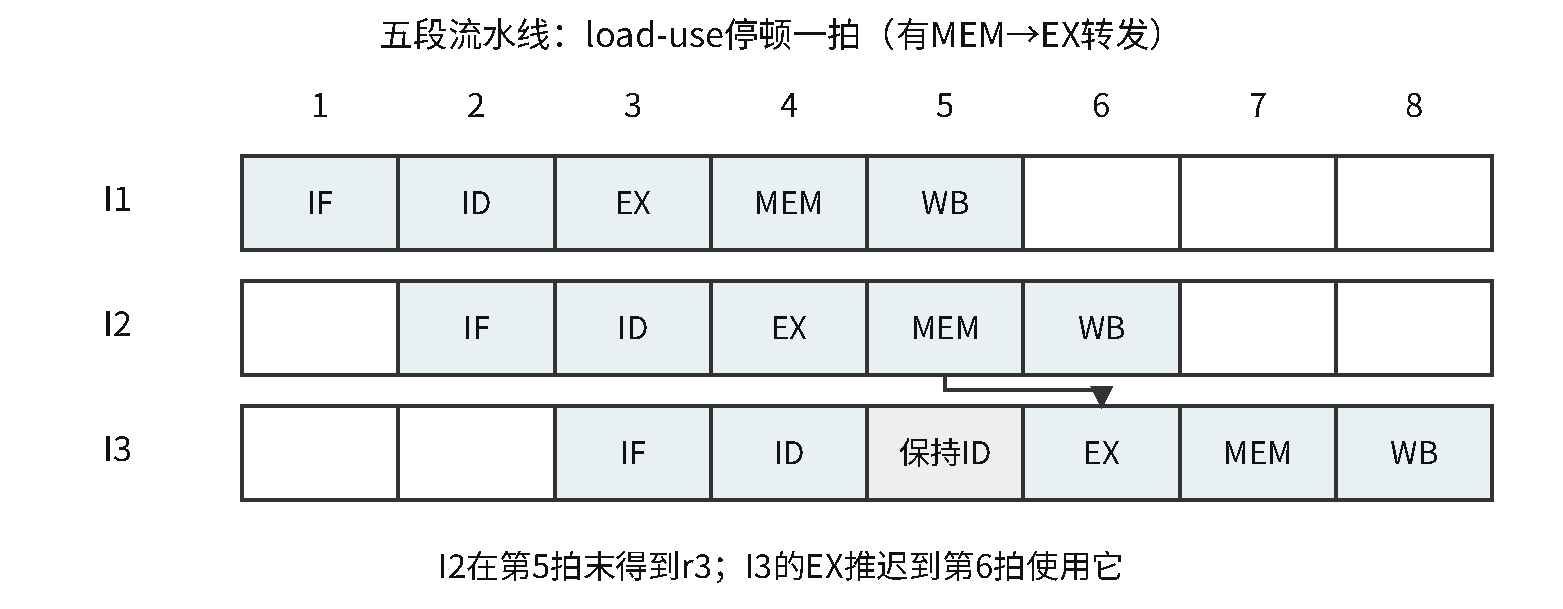
\includegraphics[width=0.96\textwidth,height=\textheight]{figures/CO_F09_pipeline_load.pdf}
\caption{load到MEM末才有数据；空泡把使用时刻推迟到下一拍}\label{co-fig-pipeline}
\end{figure}

\begin{longtable}[]{@{}
  >{\raggedright\arraybackslash}p{(\columnwidth - 16\tabcolsep) * \real{0.1111}}
  >{\raggedright\arraybackslash}p{(\columnwidth - 16\tabcolsep) * \real{0.1111}}
  >{\raggedright\arraybackslash}p{(\columnwidth - 16\tabcolsep) * \real{0.1111}}
  >{\raggedright\arraybackslash}p{(\columnwidth - 16\tabcolsep) * \real{0.1111}}
  >{\raggedright\arraybackslash}p{(\columnwidth - 16\tabcolsep) * \real{0.1111}}
  >{\raggedright\arraybackslash}p{(\columnwidth - 16\tabcolsep) * \real{0.1111}}
  >{\raggedright\arraybackslash}p{(\columnwidth - 16\tabcolsep) * \real{0.1111}}
  >{\raggedright\arraybackslash}p{(\columnwidth - 16\tabcolsep) * \real{0.1111}}
  >{\raggedright\arraybackslash}p{(\columnwidth - 16\tabcolsep) * \real{0.1111}}@{}}
\toprule\noalign{}
\begin{minipage}[b]{\linewidth}\raggedright
指令
\end{minipage} & \begin{minipage}[b]{\linewidth}\raggedright
1
\end{minipage} & \begin{minipage}[b]{\linewidth}\raggedright
2
\end{minipage} & \begin{minipage}[b]{\linewidth}\raggedright
3
\end{minipage} & \begin{minipage}[b]{\linewidth}\raggedright
4
\end{minipage} & \begin{minipage}[b]{\linewidth}\raggedright
5
\end{minipage} & \begin{minipage}[b]{\linewidth}\raggedright
6
\end{minipage} & \begin{minipage}[b]{\linewidth}\raggedright
7
\end{minipage} & \begin{minipage}[b]{\linewidth}\raggedright
8
\end{minipage} \\
\midrule\noalign{}
\endhead
\bottomrule\noalign{}
\endlastfoot
I1 & IF & ID & EX & MEM & WB & & & \\
I2 & & IF & ID & EX & MEM & WB & & \\
I3 & & & IF & ID & 保持ID & EX & MEM & WB \\
\end{longtable}

采用寄存器组同拍先写后读的时序，I1第5拍WB写回的r1可在该拍被保持在ID的I3读到；若实现不同，须另有WB到ID的旁路。第5拍EX放入气泡，I3在ID保持，下一拍接到装入结果。这里把r3的使用点设为EX，使用题目所指的常见五段转发模型；若某图要求在ID比较，所需等待和转发路径还可能不同。

\subsubsection{例 6-3　同一段序列里同时有数据与控制等待}\label{co-ex6-3}

\noindent{}【2023】 在采用``取指、译码/取数、执行、访存、写回''5段流水线的 RISC 处理器中，执行如下指令序列，其中s0、s1、s2、s3和t2表示寄存器编号。

\par\medskip\noindent
\begin{minipage}{\linewidth}
\begin{verbatim}
I1: add  s2, s1, s0  // R[s2] <- R[s1] + R[s0]
I2: load s3, 0(s2)   // R[s3] <- M[R[s2] + 0]
I3: beq  t2, s3, L1  // if R[t2] = R[s3] jump to L1
I4: addi t2, t2, 20  // R[t2] <- R[t2] + 20
I5: L1: ...
\end{verbatim}
\end{minipage}\par\medskip

若采用转发（旁路）技术处理数据冒险，采用硬件阻塞方式处理控制冒险，则在指令I1～I4的执行过程中，发生流水线阻塞的指令有（　）。

A. 仅 I3　 B. 仅 I2、I4　 C. 仅 I3、I4　 D. I2、I3、I4

\Needspace{6\baselineskip}

\textbf{解析。} I1的ALU结果可以及时转发给I2计算地址，所以I2不因这项RAW等待。I2是load，I3马上使用s3，仍有load-use等待。I3的分支结果未确定时，硬件阻塞后继I4，形成控制等待。因此为I3、I4，选 \textbf{C}。一条序列不能只找第一组相关就结束；每个使用值的位置和后继PC都要检查。

\subsubsection{三种处理办法各改变什么}\label{ux4e09ux79cdux5904ux7406ux529eux6cd5ux5404ux6539ux53d8ux4ec0ux4e48}

硬件阻塞保留相关指令及其前方必要状态，在前级暂停、后级放气泡，让生产者先前进。编译调度把不依赖该结果、且移动后不改变程序语义的指令填进等待间隔；无法填满才用NOP。不能把有副作用或可能越界访存的指令随意移过分支。

分支预测先选择一条路径继续取指，正确时减少等待，错误时清除错误路径上尚不能提交的结果并从正确位置重新取指。若每条指令发生预测错误的概率为p、每次平均损失d周期，且其他开销已包含在基本CPI中，可用 \(\mathrm{CPI}=\mathrm{CPI}_{0}+pd\)；不能把``分支比例''直接当``所有指令的预测失败比例''。

旁路主要解决值的及时可用，不直接决定分支目标地址；某些设计把数据转发给分支比较器，缩短因数据相关而产生的分支等待，但不等于所有控制冒险都由旁路消除。题目需按具体控制路径判断。

\subsection{超标量与动态流水线允许哪些重叠}\label{co-06-04}

超标量CPU每周期可发射多条指令，需要相应的译码、调度、执行和写回资源。是否真能每周期发满，取决于数据依赖、分支、功能部件和访存带宽。最大发射宽度w只给出理想吞吐上限，不能用w直接作为任意程序的加速比。

超流水把阶段划得更细，试图缩短时钟周期。阶段寄存器开销和冒险损失会限制收益。超长指令字 VLIW 把若干可并行操作交给编译器打包，硬件和指令格式仍需支持相应并行执行，并非``只改编译器，硬件没有要求''。

动态调度可让后面的就绪指令先执行，减少因前面一条长延迟指令而造成的闲置。寄存器重命名为不同逻辑写入分配不同物理位置，可去除WAR、WAW这类假相关，但不能消除真实RAW：消费者必须等对应生产者的值。按序提交进一步使软件看到的状态符合程序顺序，并帮助实现精确异常。

例如前指令还要读取旧r1，后指令将写新r1时，为新值分配另一物理寄存器，可避免覆盖旧值；若后指令确实需要前指令算出的r1，则改名字也不能凭空产生结果。区分``名字相同''和``值确有依赖''比背三组字母更有用。

\subsection{一条指令处理多个数据，还是多个指令流}\label{co-06-05}

Flynn分类按指令流和数据流区分：SISD为单指令流单数据流；SIMD为单指令流多数据流；MISD为多指令流单数据流；MIMD为多指令流多数据流。分类描述执行组织，不是按机器装了几个屏幕、几块内存来判断。

向量处理器用一条向量指令对一组数据元素重复执行同类操作，可采用向量流水和多个通道，属于常见SIMD组织。它有启动代价，长向量能更好摊薄；向量长度不等于同时存在同样多套完整处理器。SIMD也不能自然处理每个元素都要求完全不同控制流程的任务，分支发散可能降低有效利用率。

MIMD允许不同处理单元执行不同指令流。共享物理地址空间的多处理器属于MIMD的一种，分布式存储系统也可属于MIMD。SMP中的``对称''是各处理器在系统功能等方面地位对等，不表示每个时刻执行同一条指令。

\subsection{硬件线程、多核与共享内存}\label{co-06-06}

硬件多线程让一个核保存多套线程体系结构状态，以便在一个线程等待时运行另一线程。细粒度多线程可按周期交替线程；粗粒度多线程常在较长延迟事件时切换；同时多线程 SMT 允许同周期从不同线程发射操作，利用已有执行资源。它们都不要求芯片必须有多个核。

多核是在一个处理器芯片内集成多个执行核心。各核可以独立推进指令流，通常还共享某些Cache、互连或内存控制资源。增加核数不保证单线程加速，也不保证功耗必然高于任意单核设计；工艺、频率、负载和资源共享均影响结果。

共享内存多处理器让各处理器使用同一物理地址空间，但各核寄存器、部分Cache仍可私有。共享地址只保证可以指向同一对象，不保证多个读改写操作自动原子。并发程序还需要同步，Cache一致性与存储顺序也要分别满足相应规则。操作系统的进程同步讲义会沿用这一边界。

\subsubsection{例 6-4　硬件多线程不等于多核}\label{co-ex6-4}

\noindent{}【2022】 下列关于并行处理技术的叙述中，不正确的是（　）。

A. 多核处理器属于 MIMD 结构\\
B. 向量处理器属于 SIMD 结构\\
C. 硬件多线程技术只可用于多核处理器\\
D. SMP中所有处理器共享单一物理地址空间

\Needspace{6\baselineskip}

\textbf{解析。} 单核也能保存多套线程状态并共享执行部件，所以 C 错，选 \textbf{C}。A、B从指令流和数据流分类，D说的是共享物理地址空间；都没有断言所有资源完全相同或所有访问自动同步。

\subsubsection{例 6-5　无转发流水线的阻塞传播与最短调度}\label{co-ex6-5}

\noindent{}【2012】 某16位计算机中，带符号整数用补码表示，数据Cache和指令Cache分离。下面给出了指令系统中部分指令的汇编格式及对应功能，其中Rs和Rd表示寄存器，mem表示存储单元地址，(x)表示寄存器x或存储单元x的内容。

\par\medskip\noindent
\begin{minipage}{\linewidth}
\begin{verbatim}
ADD   Rs, Rd
SHL   Rd
SHR   Rd
LOAD  Rd, mem
STORE Rs, mem
\end{verbatim}
\end{minipage}\par\medskip

上面每行给出一种汇编格式；下表按助记符逐项对应其名称和功能，不改变源、目的操作数的次序。

\begin{longtable}[]{@{}
  >{\raggedright\arraybackslash}p{(\columnwidth - 4\tabcolsep) * \real{0.2874}}
  >{\raggedright\arraybackslash}p{(\columnwidth - 4\tabcolsep) * \real{0.2519}}
  >{\raggedright\arraybackslash}p{(\columnwidth - 4\tabcolsep) * \real{0.4606}}@{}}
\toprule\noalign{}
\begin{minipage}[b]{\linewidth}\raggedright
名称
\end{minipage} & \begin{minipage}[b]{\linewidth}\raggedright
助记符
\end{minipage} & \begin{minipage}[b]{\linewidth}\raggedright
指令功能
\end{minipage} \\
\midrule\noalign{}
\endhead
\bottomrule\noalign{}
\endlastfoot
加法 & \texttt{ADD} & \((\mathrm{Rs})+(\mathrm{Rd})\to\mathrm{Rd}\) \\
算术/逻辑左移 & \texttt{SHL} & \(2(\mathrm{Rd})\to\mathrm{Rd}\) \\
算术右移 & \texttt{SHR} & \((\mathrm{Rd})/2\to\mathrm{Rd}\) \\
取数 & \texttt{LOAD} & \((\mathrm{mem})\to\mathrm{Rd}\) \\
存数 & \texttt{STORE} & \((\mathrm{Rs})\to\mathrm{mem}\) \\
\end{longtable}

该计算机采用5段流水方式执行指令，各流水段分别是取指IF、译码/读寄存器ID、执行/计算有效地址EX、访问存储器M和结果写回寄存器WB。流水线采用``按序发射、按序完成''方式，没有采用转发技术处理数据相关，并且同一个寄存器的读和写操作不能在同一个时钟周期内进行。请回答下列问题。

（1）若int型变量x的值为−513，存放在寄存器R1中，则执行指令 \texttt{SHR\ R1} 后，R1的内容是多少（用十六进制表示）？

（2）若某个时间段中有连续4条指令进入流水线，在其执行过程中没有发生任何阻塞，则执行这4条指令需要多少个时钟周期？

（3）若赋值语句为 \texttt{x=a+b}，x、a、b均为int型变量，其存储单元地址分别为{[}x{]}、{[}a{]}、{[}b{]}。对应指令序列及流水过程如下，I3的ID段和I4的IF段被阻塞的原因各是什么？

\par\medskip\noindent
\begin{minipage}{\linewidth}
\begin{verbatim}
I1  LOAD  R1, [a]
I2  LOAD  R2, [b]
I3  ADD   R1, R2
I4  STORE R2, [x]
\end{verbatim}
\end{minipage}\par\medskip

\begin{longtable}[]{@{}
  >{\raggedright\arraybackslash}p{(\columnwidth - 28\tabcolsep) * \real{0.0666}}
  >{\raggedright\arraybackslash}p{(\columnwidth - 28\tabcolsep) * \real{0.0666}}
  >{\raggedright\arraybackslash}p{(\columnwidth - 28\tabcolsep) * \real{0.0666}}
  >{\raggedright\arraybackslash}p{(\columnwidth - 28\tabcolsep) * \real{0.0666}}
  >{\raggedright\arraybackslash}p{(\columnwidth - 28\tabcolsep) * \real{0.0666}}
  >{\raggedright\arraybackslash}p{(\columnwidth - 28\tabcolsep) * \real{0.0666}}
  >{\raggedright\arraybackslash}p{(\columnwidth - 28\tabcolsep) * \real{0.0666}}
  >{\raggedright\arraybackslash}p{(\columnwidth - 28\tabcolsep) * \real{0.0666}}
  >{\raggedright\arraybackslash}p{(\columnwidth - 28\tabcolsep) * \real{0.0666}}
  >{\raggedright\arraybackslash}p{(\columnwidth - 28\tabcolsep) * \real{0.0666}}
  >{\raggedright\arraybackslash}p{(\columnwidth - 28\tabcolsep) * \real{0.0666}}
  >{\raggedright\arraybackslash}p{(\columnwidth - 28\tabcolsep) * \real{0.0666}}
  >{\raggedright\arraybackslash}p{(\columnwidth - 28\tabcolsep) * \real{0.0666}}
  >{\raggedright\arraybackslash}p{(\columnwidth - 28\tabcolsep) * \real{0.0666}}
  >{\raggedright\arraybackslash}p{(\columnwidth - 28\tabcolsep) * \real{0.0666}}@{}}
\toprule\noalign{}
\begin{minipage}[b]{\linewidth}\raggedright
指令
\end{minipage} & \begin{minipage}[b]{\linewidth}\raggedright
1
\end{minipage} & \begin{minipage}[b]{\linewidth}\raggedright
2
\end{minipage} & \begin{minipage}[b]{\linewidth}\raggedright
3
\end{minipage} & \begin{minipage}[b]{\linewidth}\raggedright
4
\end{minipage} & \begin{minipage}[b]{\linewidth}\raggedright
5
\end{minipage} & \begin{minipage}[b]{\linewidth}\raggedright
6
\end{minipage} & \begin{minipage}[b]{\linewidth}\raggedright
7
\end{minipage} & \begin{minipage}[b]{\linewidth}\raggedright
8
\end{minipage} & \begin{minipage}[b]{\linewidth}\raggedright
9
\end{minipage} & \begin{minipage}[b]{\linewidth}\raggedright
10
\end{minipage} & \begin{minipage}[b]{\linewidth}\raggedright
11
\end{minipage} & \begin{minipage}[b]{\linewidth}\raggedright
12
\end{minipage} & \begin{minipage}[b]{\linewidth}\raggedright
13
\end{minipage} & \begin{minipage}[b]{\linewidth}\raggedright
14
\end{minipage} \\
\midrule\noalign{}
\endhead
\bottomrule\noalign{}
\endlastfoot
I1 & IF & ID & EX & M & WB & & & & & & & & & \\
I2 & & IF & ID & EX & M & WB & & & & & & & & \\
I3 & & & IF & & & & ID & EX & M & WB & & & & \\
I4 & & & & & & & IF & & & & ID & EX & M & WB \\
\end{longtable}

上表沿原图画法，只标每段成功推进的拍，空格不统一代表同一种状态：I3第4～6拍在ID端等待，I4第4～6拍尚未获准取指，第8～10拍又在ID端等待；这些等待格应保留。各行取指前及流出后的其他空格表示该指令尚未进入或已经离开流水线。

（4）若赋值语句为 \texttt{x=x*2+a}，x和a均为unsigned int型变量，其存储单元地址分别为{[}x{]}、{[}a{]}，执行这条语句至少需要多少个时钟周期？要求模仿上图，画出对应指令序列及流水线执行过程示意图。

\Needspace{6\baselineskip}

\textbf{解析。} 本题与例6-2的转发模型不同。统一使用约束：源寄存器若在第w拍WB写回，则消费者最早第w+1拍在ID完成取数并向后推进；在此之前可以停留于ID端等待，IF/ID寄存器保持，后继取指也被阻塞。按题中过程，所有指令均走完五段计完成，即使某一段不产生实际数据读写。

（1）−513的16位补码为 \texttt{FDFFH}，即 \texttt{1111\ 1101\ 1111\ 1111}。算术右移复制符号位，得到 \texttt{1111\ 1110\ 1111\ 1111}，即 \texttt{FEFFH}，真值−257。表中``除以2''说明算术右移的数量关系；对负奇数按位右移相当于向负无穷取整，不能代入C整数除法向零截断而答−256。

（2）无阻塞时，第一条用5拍，后3条每隔1拍完成，共 \(5+4-1=8\) 拍。指令Cache与数据Cache分离，不能额外添加题干未给的取指与数据访存争用。

（3）I3要读I1写入的R1和I2写入的R2，存在两条RAW依赖。I1在第5拍、I2在第6拍WB写回，且不许同拍读写，所以I3在第4～6拍于ID端等待，第7拍才可完成取数，而非第6拍。I3占用的IF/ID状态尚未释放时，若I4继续取指，会覆盖这条待推进指令，因此I4的IF也推迟到第7拍。后一处是前方数据等待向取指端传播，不能误说成STORE在IF就要读R2。

等I3在第10拍WB写出和，I4才可在第11拍ID读取R2，随后经过EX、M、WB，在第14拍流出。原图的两段空白应分别追到其等待的生产者与受阻资源，不能把空白一概叫作访存延迟。

（4）用两个寄存器保存x和a，让x先装入，以便尽早启动连续依赖的移位、相加：

\par\medskip\noindent
\begin{minipage}{\linewidth}
\begin{verbatim}
I1  LOAD  R1, [x]
I2  LOAD  R2, [a]
I3  SHL   R1          // 也可用 ADD R1, R1
I4  ADD   R1, R2      // R2 <- 2*x + a
I5  STORE R2, [x]
\end{verbatim}
\end{minipage}\par\medskip

\begin{figure}
\centering
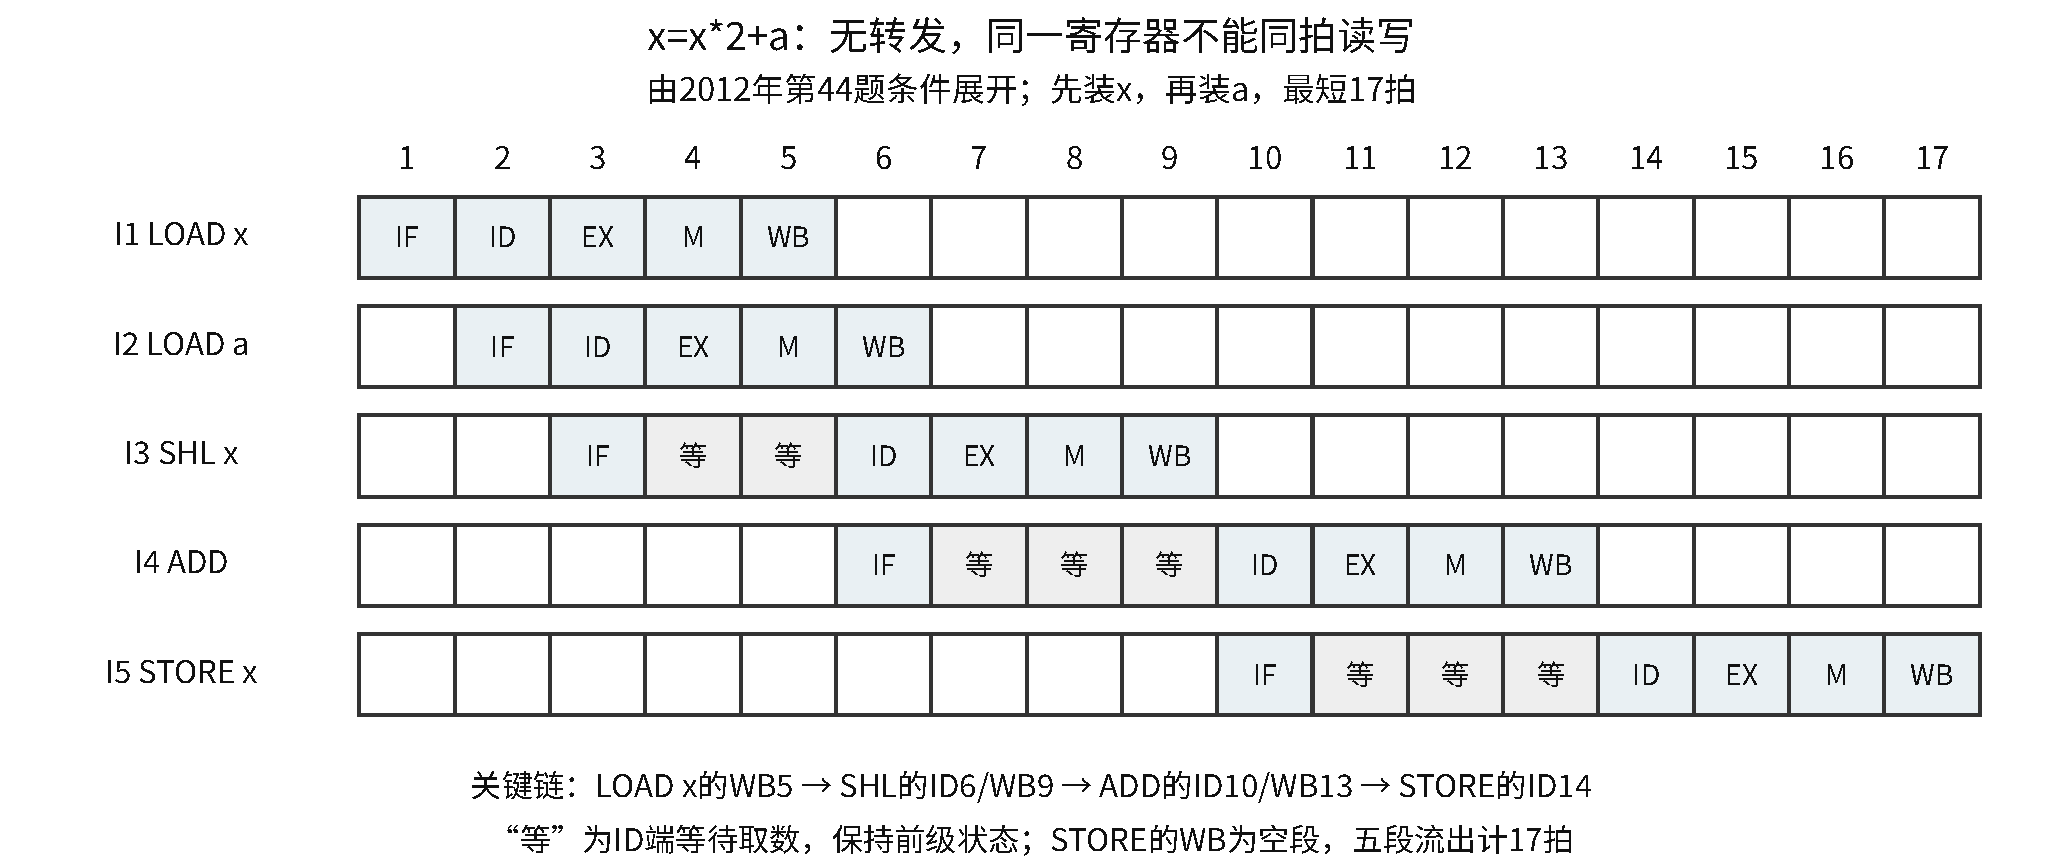
\includegraphics[width=0.98\textwidth,height=\textheight]{figures/CO_F13_pipeline_schedule.pdf}
\caption{无转发且寄存器不能同拍读写：分别等待WB后的下一拍，最短17拍}\label{co-fig-pipeline-schedule}
\end{figure}

I1第5拍WB，故I3最早第6拍ID、第9拍WB。I4依赖I3的R1，最早第10拍ID、第13拍WB；I2已在第6拍写回，不再额外拖延I4。I5最早第14拍ID，至第17拍流出，故至少17拍。

这个排程还给出了下界证明：本题给定指令中，需要两次LOAD、一次翻倍、一次相加和一次STORE；x的``LOAD→翻倍→相加→STORE''链不能颠倒。即使其余工作都尽早完成，这条链也要求上面的ID下界6、10、14；所列排程恰好达到下界。若先装a再装x，关键链反而晚一拍。STORE在第16拍M已写存储器，但按原题五段完整流出的统一口径，答案仍为17拍。

\subsubsection{自测}\label{co-self6}

\begin{enumerate}
\def\labelenumi{\arabic{enumi}.}
\tightlist
\item
  原创补充：理想5段流水线周期2 ns，完成20条指令，中间有3个导致整体延长的停顿周期，求总时间与实际吞吐率。
\item
  原创补充：若一条指令的结果要到MEM末才形成，而消费者在下一拍EX开始使用，有MEM→EX转发，是否仍需等到生产者WB结束？若消费者EX与生产者MEM是同一拍呢？
\end{enumerate}

\textbf{答案。} 1. \((5+20-1+3)\times2=54\) ns，吞吐率 \(20/54\approx0.370\) 条/ns。2. 前者不需要，可在下一拍使用MEM末的结果；后者来不及，需要推迟消费者。关键是结果形成时刻与使用时刻，而不是``二者有相关''这句判断本身。
